\documentclass[conference]{IEEEtran}
\usepackage[utf8]{inputenc}
\usepackage[T1]{fontenc}
\usepackage[spanish,es-tabla]{babel}
\usepackage{amsmath,amssymb}
\usepackage{graphicx}
\usepackage{booktabs}
\usepackage{array}
\usepackage{xcolor}
\usepackage{listings}
\usepackage{url}
\usepackage{hyperref}
\usepackage{tikz}
\usetikzlibrary{arrows.meta,positioning,babel}
\hypersetup{hidelinks}
\graphicspath{{figuras/}}
\definecolor{pendiente}{RGB}{125,54,20}
\newcommand{\completar}[1]{\textcolor{pendiente}{\textbf{[Completar: #1]}}}
\newcommand{\figpendiente}[2]{%
  \begin{figure}[!t]\centering
    \fbox{\begin{minipage}[c][31mm][c]{0.87\columnwidth}\centering\small\completar{#1}\end{minipage}}
    \caption{#2}\label{fig:#1}
  \end{figure}}
\lstdefinestyle{vhdl}{basicstyle=\ttfamily\footnotesize,breaklines=true,frame=single,columns=fullflexible,language=VHDL,showstringspaces=false}
\begin{document}
\title{Electrónica Digital 2: Laboratorio 3\\Lógica secuencial y máquinas de estados finitos}
\author{\IEEEauthorblockN{[Nombre y apellido] \qquad [Nombre y apellido] \qquad [Nombre y apellido]}
\IEEEauthorblockA{Ingeniería en Mecatrónica, Universidad Tecnológica (UTEC)\\Fray Bentos, Uruguay\\Correo: pendiente}}
\maketitle
\begin{abstract}
\completar{Redactar al finalizar: objetivo del laboratorio; divisor de 100 MHz a un pulso por segundo; contador de diez bits; FSM de cuatro operaciones; método de validación; resultados efectivamente obtenidos y principal limitación. No atribuir éxito a pruebas pendientes.}
\end{abstract}
\begin{IEEEkeywords}
FPGA, VHDL, lógica secuencial, divisor de frecuencia, contador, máquina de estados finitos, Moore, datapath, Vivado.
\end{IEEEkeywords}

\section{Introducción}
En el Laboratorio 3 de Electrónica Digital 2 se abordó el diseño de circuitos síncronos mediante VHDL sobre una FPGA Spartan-7, conforme a la consigna de la asignatura \cite{consigna}. Se plantearon dos desarrollos relacionados: en la Parte A, un divisor de frecuencia y un contador binario de diez bits; en la Parte B, una máquina de estados finitos (FSM) encargada de secuenciar operaciones lógicas y aritméticas. La habilitación temporal diseñada para la primera parte se reutilizó conceptualmente en la segunda.

La validación se dividió en simulación funcional e implementación física. \completar{Precisar aquí, en pasado, cuáles etapas se completaron realmente y cuáles quedaron sin ejecutar.}

\subsection{Objetivos}
Se establecieron los siguientes objetivos:
\begin{itemize}
\item Describir procesos síncronos en VHDL mediante \texttt{rising\_edge} y reset.
\item Calcular e implementar un divisor basado en un contador módulo \texttt{MAX}.
\item Implementar un contador ascendente con habilitación \emph{clock enable}.
\item Describir una FSM de Moore mediante estados enumerados y tres procesos.
\item Integrar la FSM como unidad de control y un \emph{datapath} combinacional.
\item Contrastar las formas de onda simuladas con el comportamiento de la FPGA.
\end{itemize}


\section{Marco teórico}
\subsection{Lógica combinacional y secuencial}
En un circuito combinacional, las salidas dependen únicamente de las entradas actuales. En uno secuencial, interviene además el estado interno, que conserva información de los ciclos anteriores \cite{cursofsm}. En VHDL, un registro se describe mediante \texttt{rising\_edge(clk)}; el reset síncrono se evalúa dentro de ese flanco, a diferencia del reset asíncrono, que puede actuar sin esperar al reloj \cite{ug901}. 

\subsection{División de frecuencia y habilitación}
Un divisor por módulo se obtuvo mediante una cuenta interna y la detección del valor terminal (\emph{terminal count}) \cite{cursodiv}. Para la práctica se especificó un pulso \texttt{en} de un ciclo de duración cada \texttt{MAX} ciclos del reloj principal. El número de ciclos requerido se calculó como
\begin{equation}
\mathrm{MAX}=\frac{f_{\mathrm{clk}}}{f_{\mathrm{pulso}}}.
\label{eq:max}
\end{equation}
De este modo, los módulos conservaron el dominio de reloj de 100 MHz y utilizaron \texttt{en} para determinar cuándo actualizar su estado. El uso de un único dominio de reloj evitó utilizar una salida lógica como reloj de otro bloque, práctica desaconsejada en FPGA por las dificultades de ruteo y análisis temporal \cite{cursodiv}. Este pulso de habilitación no fue una señal cuadrada de 1 Hz: su período fue de un segundo y su duración en alto fue de un único ciclo de 10 ns.

\subsection{FSM de Moore y datapath}
Una FSM está formada por un conjunto finito de estados, reglas de transición y salidas \cite{cursofsm}. En una máquina de Moore, las salidas dependen del estado registrado; en una de Mealy, pueden depender del estado y de las entradas actuales. La enseñanza del curso propuso un patrón de tres procesos: registro de estado síncrono, próximo estado combinacional y salida combinacional \cite{cursofsm}. En la Parte B se especificó la codificación Moore \texttt{op} correspondiente a cuatro estados; el \emph{datapath}, de naturaleza combinacional, recibió A, B y \texttt{op}. Por tanto, la salida \texttt{op} depende solo del estado, mientras que el resultado de cálculo también depende de A y B.


\section{Metodología}
\subsection{Materiales y herramientas}
Fueron utilizados la Spartan Edge Accelerator Board con dispositivo XC7S15FTGB196-1, el shield UTEC de doce entradas y diez LEDs, alimentación USB y un programador JTAG HS2. El desarrollo, la simulación XSim y la implementación fueron realizados con Vivado 2025.1.

\subsection{Parte A: divisor de frecuencia}
Se diseñó la interfaz del módulo \texttt{divisor} con entradas \texttt{clk} y \texttt{rst}, salida \texttt{en} y genérico \texttt{MAX}. Se especificó un contador interno que se reiniciaba al alcanzar \(\mathrm{MAX}-1\) y activaba \texttt{en} durante un único ciclo. Para un reloj de 100 MHz y un pulso por segundo, se obtuvo
\begin{equation}
\mathrm{MAX}_{1\,\mathrm{Hz}}=\frac{100\times10^6}{1}=100\,000\,000.
\end{equation}
Para obtener 1 kHz, el valor correspondiente fue \(\mathrm{MAX}_{1\,\mathrm{kHz}}=100\,000\). El contador interno del divisor de 1 Hz requirió \(\lceil\log_2(100\,000\,000)\rceil=27\) bits. El valor terminal se estableció en \(\mathrm{MAX}-1\), no en \(\mathrm{MAX}\), para evitar un ciclo adicional.

\subsection{Parte A: contador e integración}
Se definió un contador ascendente con genérico \texttt{N=10}, reset síncrono y habilitación \texttt{en}. Su salida \texttt{q(9 downto 0)} se asignó a los diez LEDs, con \texttt{LED0} como bit menos significativo. En el módulo superior, la salida \texttt{en} del divisor se conectó a la entrada homónima del contador. Así, el registro solamente incrementaba cuando recibía un pulso de habilitación. El rango de diez bits fue de 0 a 1023, seguido de desborde a cero.

La Fig.~\ref{fig:bloquesA} muestra las conexiones del top de la Parte A.
\begin{figure*}[!t]\centering
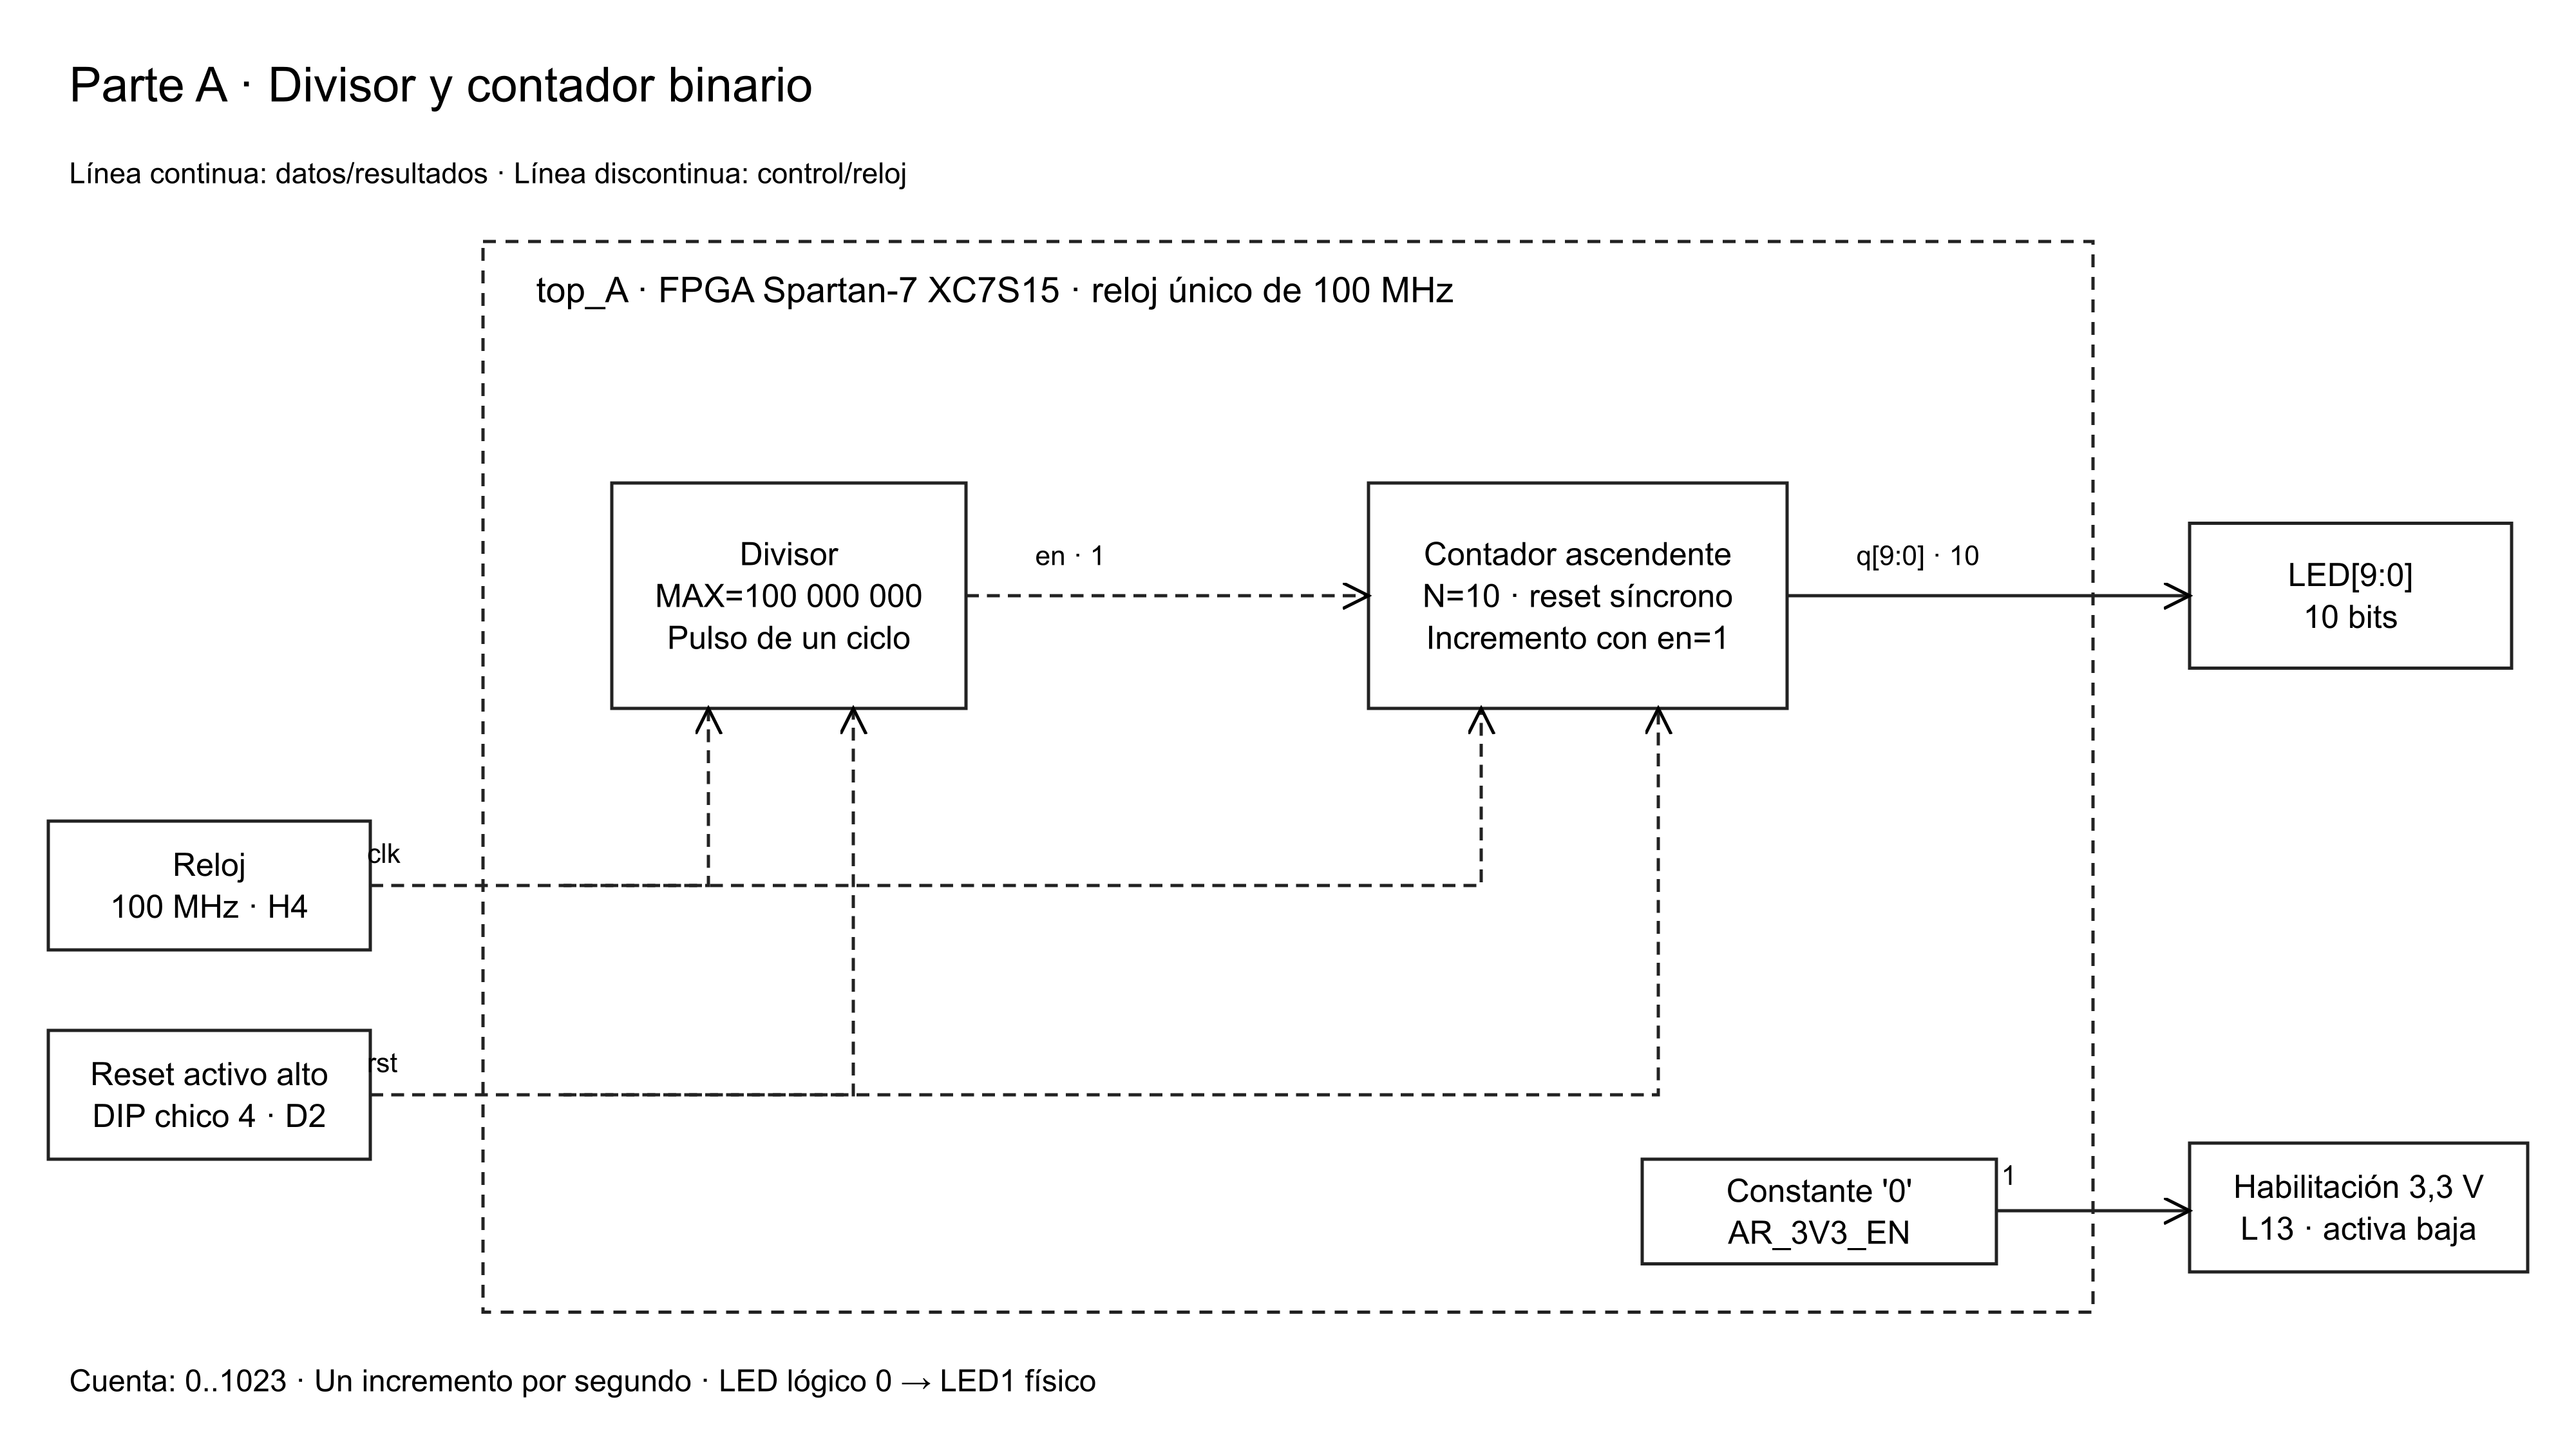
\includegraphics[width=\textwidth]{parte_a_integracion.png}
\caption{Integración de la Parte A: divisor y contador bajo un único reloj, reset común y salida de diez bits hacia los LEDs.}\label{fig:bloquesA}
\end{figure*}

\subsection{Comportamiento temporal esperado}
El pulso \texttt{en} fue especificado como una habilitación de un único ciclo de reloj cada \texttt{MAX} ciclos. Con \texttt{MAX=4}, la separación entre dos activaciones consecutivas fue de cuatro períodos de reloj. Con \texttt{MAX=100\,000\,000} y reloj de 100 MHz, el intervalo fue de un segundo. En un contador binario, cada bit dividió por dos la frecuencia de la señal cuadrada representada por el bit inmediato inferior \cite{cursodiv}. El avance de la cuenta permaneció sujeto a \texttt{en}, no a un flanco de una señal generada por lógica combinacional.

\subsection{Parte B: FSM y diagrama de estados}
Se definieron los estados enumerados \texttt{S\_AND}, \texttt{S\_OR}, \texttt{S\_XOR} y \texttt{S\_ADD}. Cada pulso de habilitación provocó, por especificación, una transición al siguiente estado y, después de \texttt{S\_ADD}, el retorno a \texttt{S\_AND}. El reset se definió con destino \texttt{S\_AND}. Se separaron el registro de estado, la lógica combinacional del próximo estado y la decodificación de la salida \texttt{op}, siguiendo el patrón de tres procesos presentado en el material del curso \cite{cursofsm}. La habilitación se consideró dentro de la lógica de transición o del registro, sin generar un segundo reloj.

\begin{figure}[!t]
\centering
\begin{tikzpicture}[>=Stealth, every node/.style={font=\scriptsize}, st/.style={draw,rounded corners,minimum width=18mm,minimum height=8mm,align=center}, node distance=12mm and 10mm]
\node[st] (a) {S\_AND\\00};
\node[st,right=of a] (b) {S\_OR\\01};
\node[st,below=of b] (c) {S\_XOR\\10};
\node[st,left=of c] (d) {S\_ADD\\11};
\draw[->] (a) -- node[above]{en} (b);
\draw[->] (b) -- node[right]{en} (c);
\draw[->] (c) -- node[below]{en} (d);
\draw[->] (d) -- node[left]{en} (a);
\draw[->] ([xshift=-10mm]a.west) -- node[above]{reset} (a.west);
\path (a) edge[loop above,->] node{sin en} (a)
(b) edge[loop above,->] node{sin en} (b)
(c) edge[loop below,->] node{sin en} (c)
(d) edge[loop below,->] node{sin en} (d);
\end{tikzpicture}
\caption{Diagrama de estados de la FSM implementada. El reset tuvo prioridad sobre la habilitación y estableció S\_AND desde cualquier estado.}\label{fig:fsm}
\end{figure}

\subsection{Parte B: datapath e integración}
El datapath recibió \texttt{A(3:0)}, \texttt{B(3:0)} y \texttt{op(1:0)}. Se definieron las operaciones y la visualización indicadas en la Tabla~\ref{tab:ops}. La suma se representó en cinco bits para conservar el acarreo, mientras que las operaciones lógicas se expresaron en cuatro bits. El divisor de la Parte A fue incorporado como fuente de habilitación para la FSM.

\begin{table}[!t]
\centering\caption{Codificación y salidas de la Parte B}\label{tab:ops}
\begin{tabular}{@{}lllp{0.28\columnwidth}@{}}\toprule
\textbf{op} & \textbf{Estado} & \textbf{Cálculo} & \textbf{Salidas}\\\midrule
00 & AND & \(A\land B\) & LED3:0\\
01 & OR & \(A\lor B\) & LED3:0\\
10 & XOR & \(A\oplus B\) & LED3:0\\
11 & ADD & \(A+B\) & LED4:0\\\bottomrule
\end{tabular}
\end{table}

\begin{figure*}[!t]
\centering
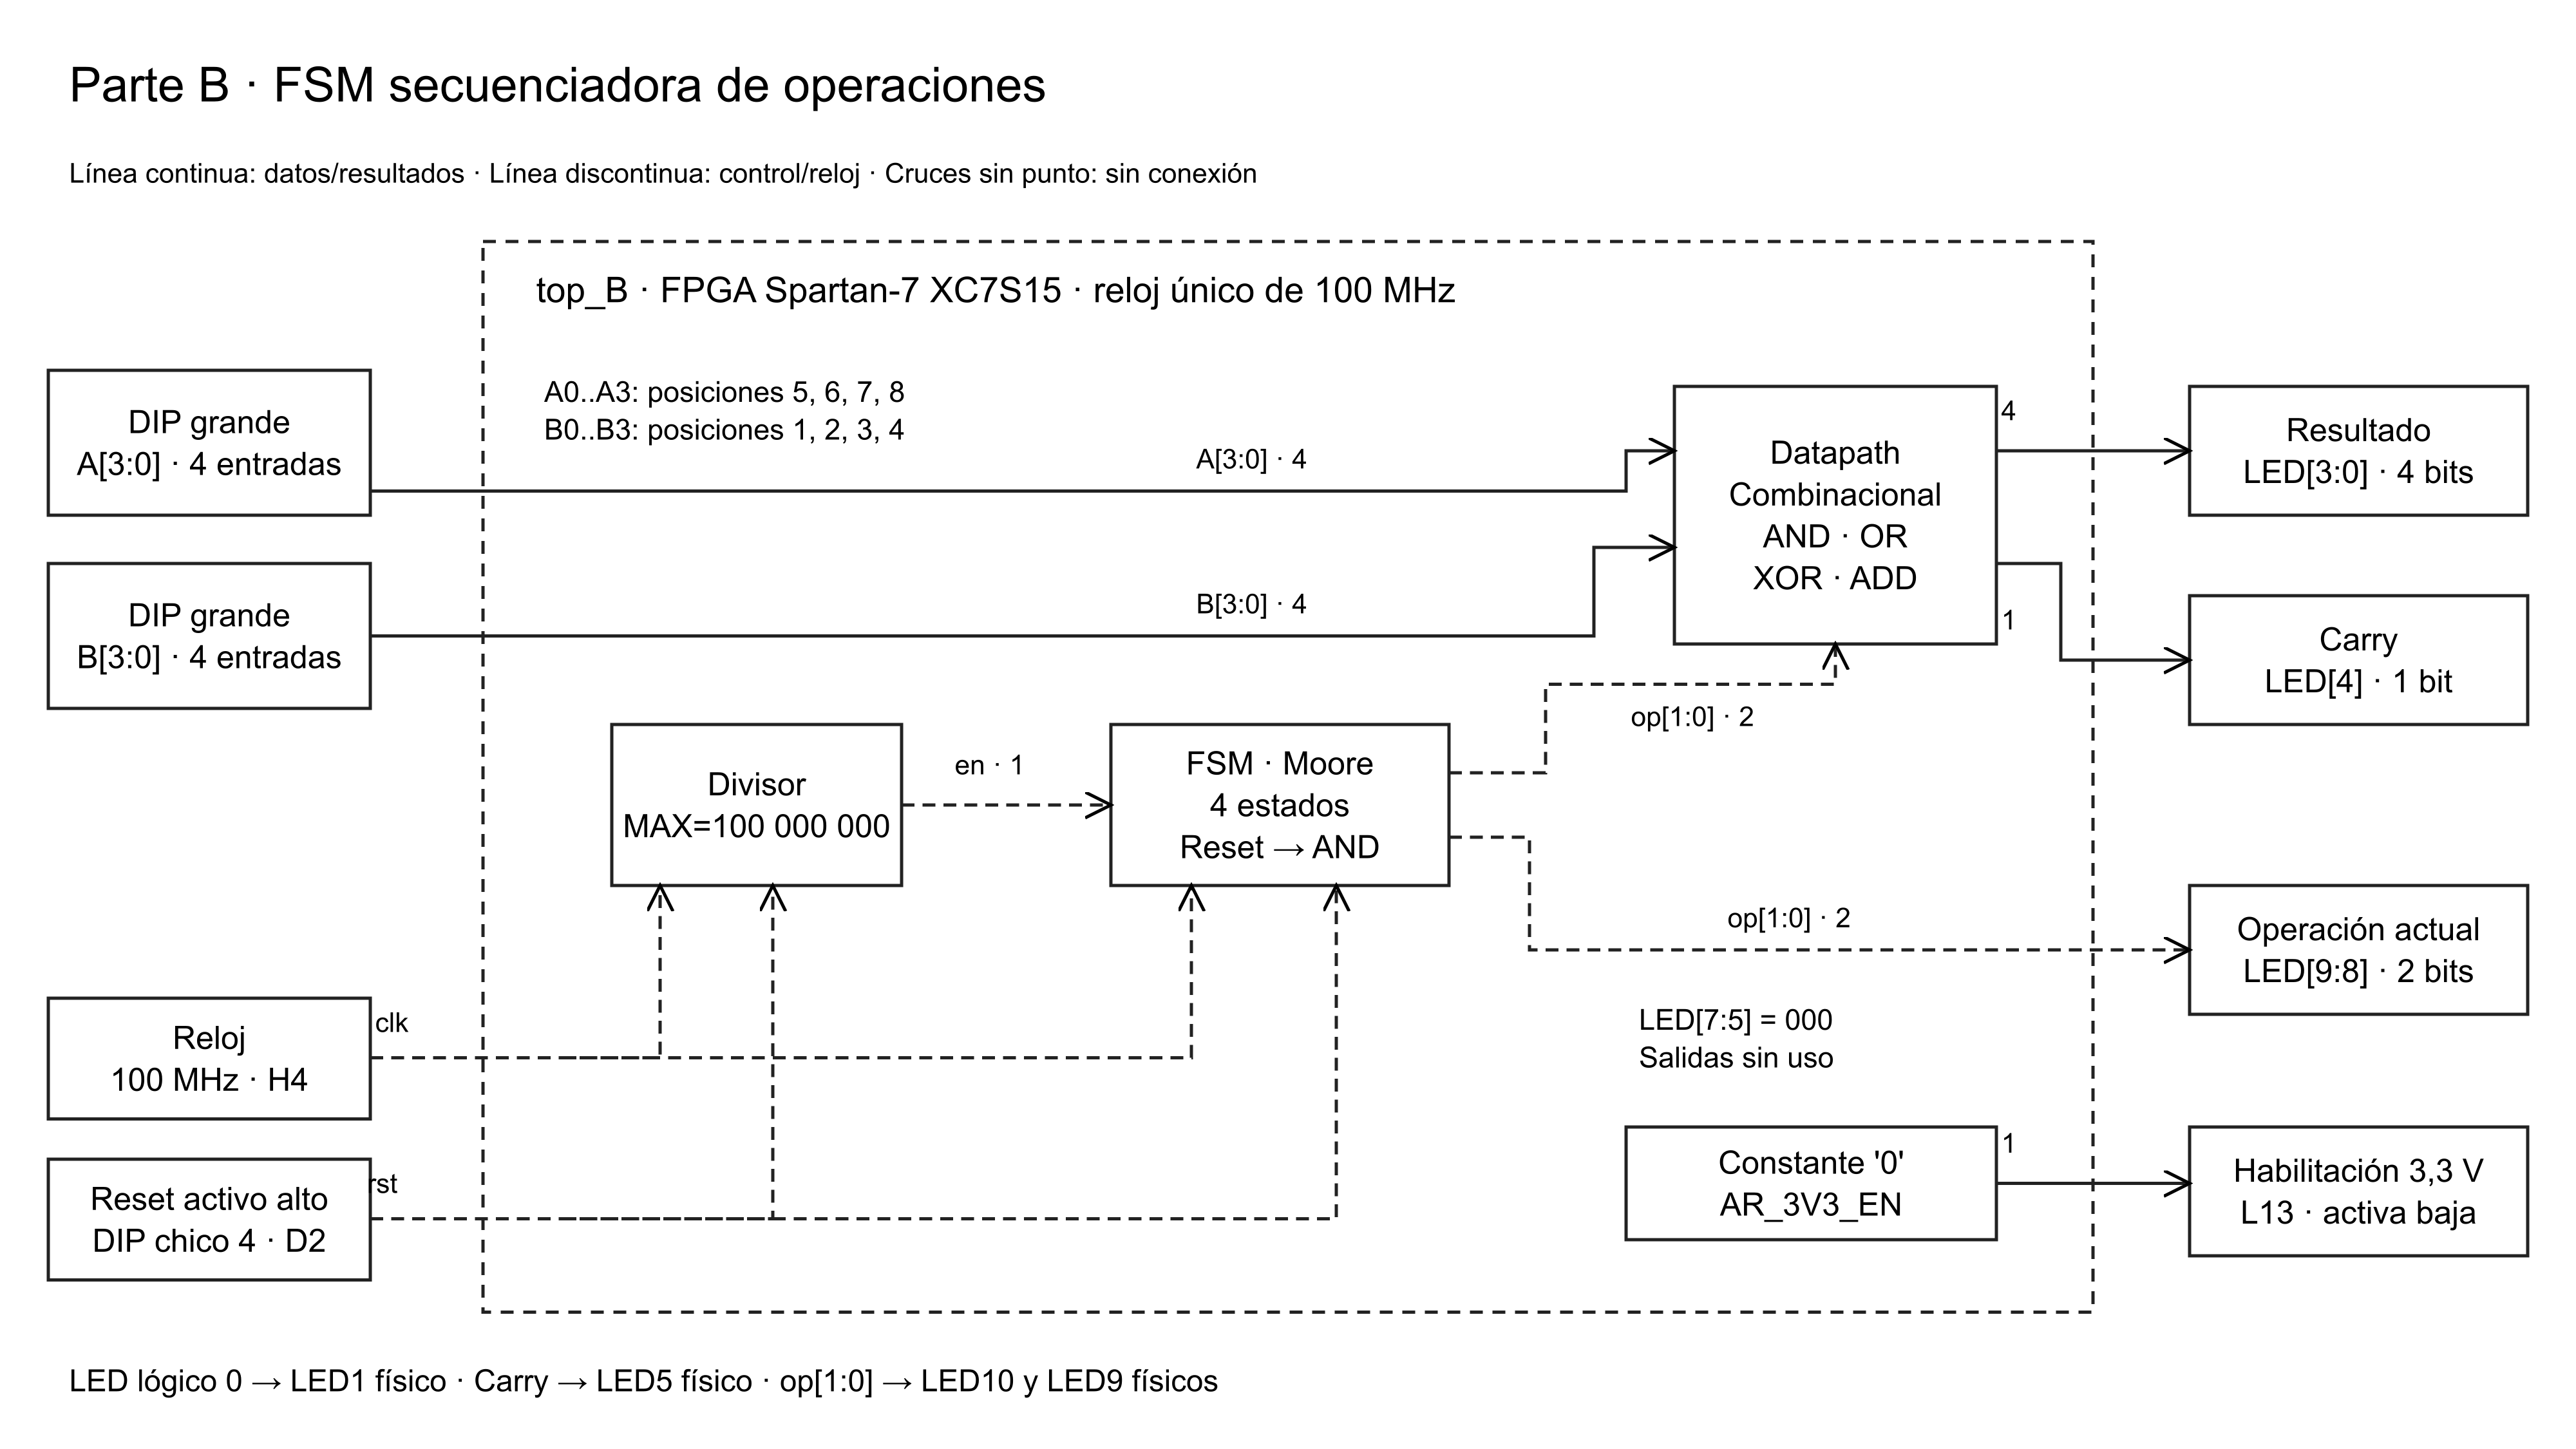
\includegraphics[width=\textwidth]{parte_b_integracion.png}
\caption{Integración de la Parte B: entradas A y B, divisor, FSM, datapath y salidas. El reloj y el reset fueron comunes al divisor y a la FSM; las salidas LED[7:5] fueron fijadas a cero.}\label{fig:bloques}
\end{figure*}

\subsection{Simulación y testbenches}
Para la Parte A se planteó un escenario de prueba con \texttt{MAX=4}, que permitió observar los pulsos sin simular cien millones de ciclos entre habilitaciones. Se fijaron como criterios de verificación la duración de un ciclo de \texttt{en}, su periodicidad, el incremento unitario, el desborde y el reset. En el material de clase se recomendó medir períodos entre eventos con \texttt{now} y utilizar \texttt{assert}; al comparar valores después de un flanco, se propuso un retardo breve para permitir la actualización de los ciclos delta del simulador \cite{cursodiv}. Para la Parte B se establecieron dos recorridos completos de la secuencia, un reset desde un estado distinto de \texttt{S\_AND} y casos de prueba para cada operación, incluida una suma con acarreo. El material de FSM mostró la comparación de salidas esperadas mediante \texttt{assert}, práctica aplicable a la secuencia de \texttt{op} \cite{cursofsm}. La periodicidad de en, la cuenta, el desborde y el reset fueron comprobados mediante assert en la Parte A; la secuencia, la retención, el reset y todos los pares de operandos por operación fueron comprobados mediante assert en la Parte B. Las capturas fueron utilizadas como evidencia visual complementaria.

\subsection{Restricciones e implementación en la placa}
La consigna estableció el reloj de 100 MHz en el pin H4 y requirió la restricción temporal \texttt{create\_clock}. Las entradas y salidas del shield utilizaron el estándar \texttt{LVCMOS33}. Además, la salida \texttt{AR\_3V3\_EN} quedó definida como activa en bajo, con asignación al pin L13 y valor lógico cero para habilitar la alimentación de los dip-switches \cite{consigna}. Se cotejaron las conexiones con el esquema del shield y el XDC maestro de la SEA. El reset se asignó a D2 (A10), posición 4 del DIP chico. Los operandos se agruparon en el DIP grande: A[0:3] en posiciones 5,6,7,8 y B[0:3] en posiciones 1,2,3,4. En la Parte B, A[0:3] se conectó a D9,D8,D7,D6 (A2, B3, A3, A4) y B[0:3] a D13,D12,D11,D10 (H2, H1, B1, B2). Los diez LEDs físicos, LED1 a LED10, se conectaron a LED[0] a LED[9], respectivamente, mediante FPGAIO9 a FPGAIO0. Se completaron síntesis, colocación y ruteo de ambas partes en Vivado 2025.1 para el dispositivo XC7S15FTGB196-1. Se programaron ambas partes por JTAG. La validación física y su registro se documentaron en la sección de resultados.


La Tabla~\ref{tab:dipfinal} resume la asignación física final utilizada en las pruebas.
\begin{table}[!t]
\centering\caption{Asignación final de los DIP-switches}\label{tab:dipfinal}
\begin{tabular}{@{}llll@{}}\toprule
Señal & DIP/posición & Arduino & FPGA\\\midrule
rst & Chico 4 & D2 & A10\\
A0 & Grande 5 & D9 & A2\\
A1 & Grande 6 & D8 & B3\\
A2 & Grande 7 & D7 & A3\\
A3 (MSB) & Grande 8 & D6 & A4\\
B0 & Grande 1 & D13 & H2\\
B1 & Grande 2 & D12 & H1\\
B2 & Grande 3 & D11 & B1\\
B3 (MSB) & Grande 4 & D10 & B2\\\bottomrule
\end{tabular}
\end{table}

\section{Resultados y discusión}
\subsection{Parte A: simulación}
Se recibieron y revisaron los módulos \texttt{divisor}, \texttt{contador} y \texttt{top\_A}, el archivo de restricciones y el testbench \texttt{tb\_parte\_A}. Los cuatro archivos VHDL se analizaron con Vivado 2025.1 y se ejecutó el testbench con XSim. La simulación utilizó un reloj de 10 ns, \texttt{MAX=4} y un contador de tres bits para observar el desborde en un intervalo breve.

Durante 36 ciclos se compararon mediante \texttt{assert} el valor de \texttt{en} con un modelo de periodicidad y el valor del contador con una cuenta de referencia. Se verificaron el pulso de un ciclo cada cuatro ciclos, la retención entre habilitaciones, el incremento, el desborde de siete a cero y el reset inicial y durante la cuenta. La ejecución finalizó a los 385,001 ns con el mensaje de comprobaciones correctas, sin errores de aserción. En ese intervalo se consumieron ocho habilitaciones; el noveno pulso se generó al final del bucle y fue seguido por reset. El contador consume el enable registrado en el flanco anterior, por lo que su actualización ocurre un ciclo después de generarse el pulso.

Esta prueba ejercitó divisor y contador; el top de diez bits fue analizado, pero no fue la unidad instanciada por el testbench. La simulación no acredita funcionamiento físico ni valida el mapeo de pines del shield.
\completar{Incorporar captura legible de las formas de onda de esta ejecución.}

\subsection{Parte A: funcionamiento físico}
\completar{Registrar los valores observados durante al menos diez segundos, la conmutación de LED0, el incremento cada segundo y el comportamiento del reset. Si no se implementó, indicar expresamente la limitación.}

\subsection{Parte B: simulación}
\completar{Insertar captura de al menos dos ciclos de la FSM; identificar clk, rst, en, op, A, B, resultado y carry. Analizar reset y sumas con acarreo.}
\begin{figure}[!t]\centering
\fbox{\begin{minipage}[c][25mm][c]{0.85\columnwidth}\centering\small Captura de la simulación de la Parte B\end{minipage}}
\caption{Transiciones de la FSM y salidas del datapath. Imagen pendiente de incorporación.}\label{fig:simB}
\end{figure}

\subsection{Parte B: validación física}
\completar{Describir valores A y B usados, secuencia visible en LED9:8, resultado en LED3:0, carry en LED4 y reset. Comparar lo esperado con lo observado, sin marcar como verificados los casos aún no ensayados.}

\begin{table}[!t]
\centering\caption{Registro de pruebas de la FSM y del datapath}\label{tab:pruebas}
\begin{tabular}{@{}ccccc@{}}\toprule
\textbf{A} & \textbf{B} & \textbf{op} & \textbf{Esperado} & \textbf{Observado}\\\midrule
0101 & 0011 & 00 & 00001 & --\\
0101 & 0011 & 01 & 00111 & --\\
0101 & 0011 & 10 & 00110 & --\\
0101 & 0011 & 11 & 01000 & --\\
1111 & 0011 & 11 & 10010 & --\\\bottomrule
\end{tabular}
\end{table}
La Tabla~\ref{tab:pruebas} presenta casos de referencia calculados, no mediciones. El campo observado quedó sin completar hasta su contrastación experimental. Los cinco bits de salida se representaron como \texttt{LED4:0}.

\subsection{Discusión y limitaciones}
\completar{Analizar diferencias entre simulación y placa, problemas concretos de restricciones, síntesis, lectura de switches o temporización; explicar sus causas y las soluciones efectivamente aplicadas. Valorar la legibilidad del video e indicar si las tomas permitieron verificar las entradas y salidas.}


\section{Preguntas del laboratorio}
\subsection{Parte A}
\subsubsection{Circuito combinacional, secuencial y proceso síncrono}
La distinción principal fue la presencia de memoria: un circuito combinacional entregó una función de las entradas presentes y uno secuencial conservó un estado entre ciclos. En VHDL, \texttt{rising\_edge(clk)} delimitó el instante de actualización de los registros. Con reset síncrono, su acción quedó sujeta al mismo flanco, lo que hizo posible un comportamiento temporal determinista.

\subsubsection{MAX para 1 Hz y 1 kHz y anchura del contador}
Aplicando la Ec.~\eqref{eq:max}, se obtuvo \(\mathrm{MAX}_{1\,\mathrm{Hz}}=100\,000\,000\) y \(\mathrm{MAX}_{1\,\mathrm{kHz}}=100\,000\). Para representar los valores comprendidos entre cero y \(99\,999\,999\), fueron suficientes 27 bits porque \(2^{26}=67\,108\,864<100\,000\,000\leq 2^{27}=134\,217\,728\).

\subsubsection{Habilitación en lugar de reloj dividido}
El empleo de \texttt{clock enable} mantuvo el contador y el divisor sincronizados con el mismo reloj físico. Así se evitó tratar una señal generada por lógica ordinaria como una nueva red de reloj, lo que habría complicado la distribución, las restricciones temporales y el análisis de cruces entre dominios. La operación de un registro quedó condicionada a \texttt{en='1'} sin alterar su fuente de reloj.

\subsubsection{Uso de genéricos en simulación}
Con el valor real de cien millones de ciclos por pulso, una simulación de varios incrementos implicaría una cantidad muy elevada de eventos, tal como se explicó en el caso de estudio del material de divisores \cite{cursodiv}. El parámetro genérico \texttt{MAX} permitió sustituir el valor de implementación por uno pequeño, como cuatro, sin modificar la estructura lógica. En el testbench de A fueron utilizados MAX=4 y N=3, y las comprobaciones finalizaron a los 455,001 ns.

\subsubsection{Frecuencia de conmutación de los LEDs}
Para incrementos a 1 Hz, el bit \(i\) del contador cambió de nivel cada \(2^i\) segundos, y completó un período de encendido y apagado cada \(2^{i+1}\) segundos. En consecuencia, su frecuencia de señal cuadrada fue
\begin{equation}
f_{\mathrm{LED}i}=\frac{1\,\mathrm{Hz}}{2^{i+1}}.
\end{equation}
Por ejemplo, \texttt{LED0} tuvo una frecuencia de señal de 0,5 Hz (una transición por segundo), \texttt{LED1} de 0,25 Hz y \texttt{LED9} de \(1/1024\) Hz. Esta distinción evitó confundir la frecuencia de incremento del contador con la frecuencia de parpadeo de cada LED.

\subsection{Parte B}
\subsubsection{Definición y componentes de la FSM}
La FSM se representó mediante un registro de estado, una lógica de transición y una función de salida. Los cuatro estados de la Fig.~\ref{fig:fsm} representaron, en orden, AND, OR, XOR y ADD. Cada habilitación especificó el paso siguiente; después de ADD se regresó a AND. El reset estableció el estado inicial AND.

\subsubsection{Diferencia entre Moore y Mealy}
En una máquina de Moore, la salida codificada depende exclusivamente del estado almacenado; en una máquina de Mealy, también puede depender de las entradas actuales. La FSM propuesta fue de Moore porque \texttt{op} se obtuvo del estado. Aunque los resultados del datapath variaron combinacionalmente al modificarse A o B, ello no convirtió a la FSM de control en una máquina de Mealy.

\subsubsection{Estados enumerados y síntesis}
La descripción mediante un tipo enumerado permitió utilizar nombres semánticos y redujo errores asociados a códigos binarios asignados manualmente. En general, la síntesis transforma los estados simbólicos a una representación física apropiada y puede escoger una codificación distinta de la codificación de salida \texttt{op}, según sus opciones de optimización. Por tanto, la numeración de \texttt{op} no implicó necesariamente que el registro físico de estado utilizara exactamente esos dos bits.

\subsubsection{Separación de procesos síncronos y combinacionales}
El registro de estado se planteó en un proceso síncrono para conservar el estado entre flancos y actualizarlo solamente al recibirse una habilitación. La lógica de próximo estado se planteó combinacionalmente para evaluar las reglas de transición en función del estado actual. La salida de Moore se definió como función combinacional de ese estado. En el registro de la FSM fue utilizada la condición \texttt{elsif en='1' then estado <= siguiente;} dentro de \texttt{rising\_edge(clk)}, con prioridad del reset. En procesos \texttt{process(all)} separados fueron definidas las transiciones mediante \texttt{case estado} y la decodificación de \texttt{op}. De ese modo no se crearon registros adicionales en la lógica combinacional.

\subsubsection{Relación con la arquitectura de un procesador}
La FSM cumplió una función de control al seleccionar la operación mediante \texttt{op}. El datapath realizó las transformaciones de datos sobre A y B y generó los resultados. Esta separación fue análoga, en una escala sencilla, a la organización de un procesador: la unidad de control determina la acción y la ruta de datos la ejecuta. La arquitectura del laboratorio no constituyó un procesador completo, ya que no incorporó un programa de instrucciones ni todos sus registros y rutas de acceso.


\section{Conclusiones}
Fue verificada la reutilización de una habilitación periódica para controlar dos comportamientos secuenciales distintos: la cuenta binaria y el avance de una FSM. La secuencia observada en placa fue consistente con las simulaciones, mientras que el reloj de 100 MHz fue mantenido como único dominio en ambos diseños. La división temporal fue lograda mediante clock enable, sin utilizar una salida lógica como reloj adicional.

La separación entre control y datapath fue validada al mantenerse el código de operación independiente de los operandos. Para A=5 y B=3 fueron obtenidos los resultados 1, 7, 6 y 8; en la suma 15+3 fue preservado el quinto bit, con lo que fue evitada la pérdida del acarreo. El reset de la FSM fue distinguido del borrado de datos: se regresó a AND, pero los operandos permanecieron definidos por los switches.

La cobertura de prueba fue mejorada al detectarse que un reset aplicado sobre una cuenta ya nula no demostraba el comportamiento buscado. También fue comprobado que una verificación exhaustiva podía ser correcta y, a la vez, poco clara visualmente; por ello fue añadida una prueba estable de acarreo. La reorganización de los DIP redujo la ambigüedad de lectura de entradas. Como mejora posterior fue identificada la incorporación de sincronización de switches y un registro sistemático de las pruebas físicas. Los márgenes temporales internos positivos y el DRC sin violaciones respaldaron la implementación, aunque no sustituyeron la comprobación del hardware ni una medición instrumental del período.

\section*{Evidencias y archivos}
Los archivos de entrega fueron organizados en fuentes de la Parte A (divisor, contador y top), fuentes de la Parte B (FSM, datapath y top), testbenches y restricciones XDC. Las capturas de simulación fueron incorporadas en las Figs.~\ref{fig:simA}--\ref{fig:carry}. Fueron conservadas una toma de placa de la Parte A y dos de la Parte B. Al cierre de esta versión, la edición de los dos videos finales con sus segmentos de simulación y la incorporación de sus enlaces de entrega permanecieron pendientes.

\begin{thebibliography}{9}
\bibitem{consigna} Universidad Tecnológica (UTEC), ``Laboratorio 3: Lógica secuencial y máquinas de estados finitos, Partes A y B,'' Electrónica Digital 2, guía de laboratorio, 2026.
\bibitem{rubrica} Universidad Tecnológica (UTEC), ``Rúbrica de evaluación por niveles de logro: Laboratorio 3,'' Electrónica Digital 2, 2026.
\bibitem{cursodiv} Universidad Tecnológica (UTEC), \emph{Todo divisor de frecuencia es, en el fondo, un contador}, material didáctico de Electrónica Digital 2, s. f.
\bibitem{cursofsm} Universidad Tecnológica (UTEC), \emph{Sistemas que se comportan distinto según su historia}, material didáctico de Electrónica Digital 2, s. f.
\bibitem{ug901} AMD, \emph{Vivado Design Suite User Guide: Synthesis (UG901)}. [En línea]. Disponible: \url{https://docs.amd.com/r/en-US/ug901-vivado-synthesis}
\bibitem{ug900} AMD, \emph{Vivado Design Suite User Guide: Logic Simulation (UG900)}. [En línea]. Disponible: \url{https://docs.amd.com/r/en-US/ug900-vivado-logic-simulation}
\bibitem{ug903} AMD, \emph{Vivado Design Suite User Guide: Using Constraints (UG903)}. [En línea]. Disponible: \url{https://docs.amd.com/r/en-US/ug903-vivado-using-constraints}
\end{thebibliography}


\end{document}
